\documentclass{beamer}
\usepackage{amsmath}
\usepackage{graphicx}
\usepackage{subfig}
\usepackage[style=verbose]{biblatex}

\makeatletter
\let\@@magyar@captionfix\relax
\makeatother

\bibliography{../link.bib}
\renewcommand{\footnotesize}{\tiny}
\title{Latent Variable Machine Learning Algorithms: Applications in a Nuclear Physics Experiment
}
\author{Robert Solli}
\institute{University of Oslo, Expert Analytics AS}
\date{\today}

\begin{document}
\begin{frame}[t]{Masters Presentation}
	\titlepage
\end{frame}

\begin{frame}[t]{Outline}
	\begin{enumerate}
		\item Introducing the Active Target Time Projection Chamber (AT-TPC)
		\item Challenges with traditional analysis of AT-TPC data - and the evangilization of Machine Learning
			\begin{enumerate}[(i)]
				\item Recap of central literature 
				\item Introducing thesis problem statements
			\end{enumerate}
		\item An introduction to central Machine Learning concepts
		\item The Auto-Encoder neural network
		\item Results 
		\item Discussion, Summary, Conclusion and Outlook
	\end{enumerate}
\end{frame}

\begin{frame}[t]{AT-TPC}
	\begin{figure}
		\centering
		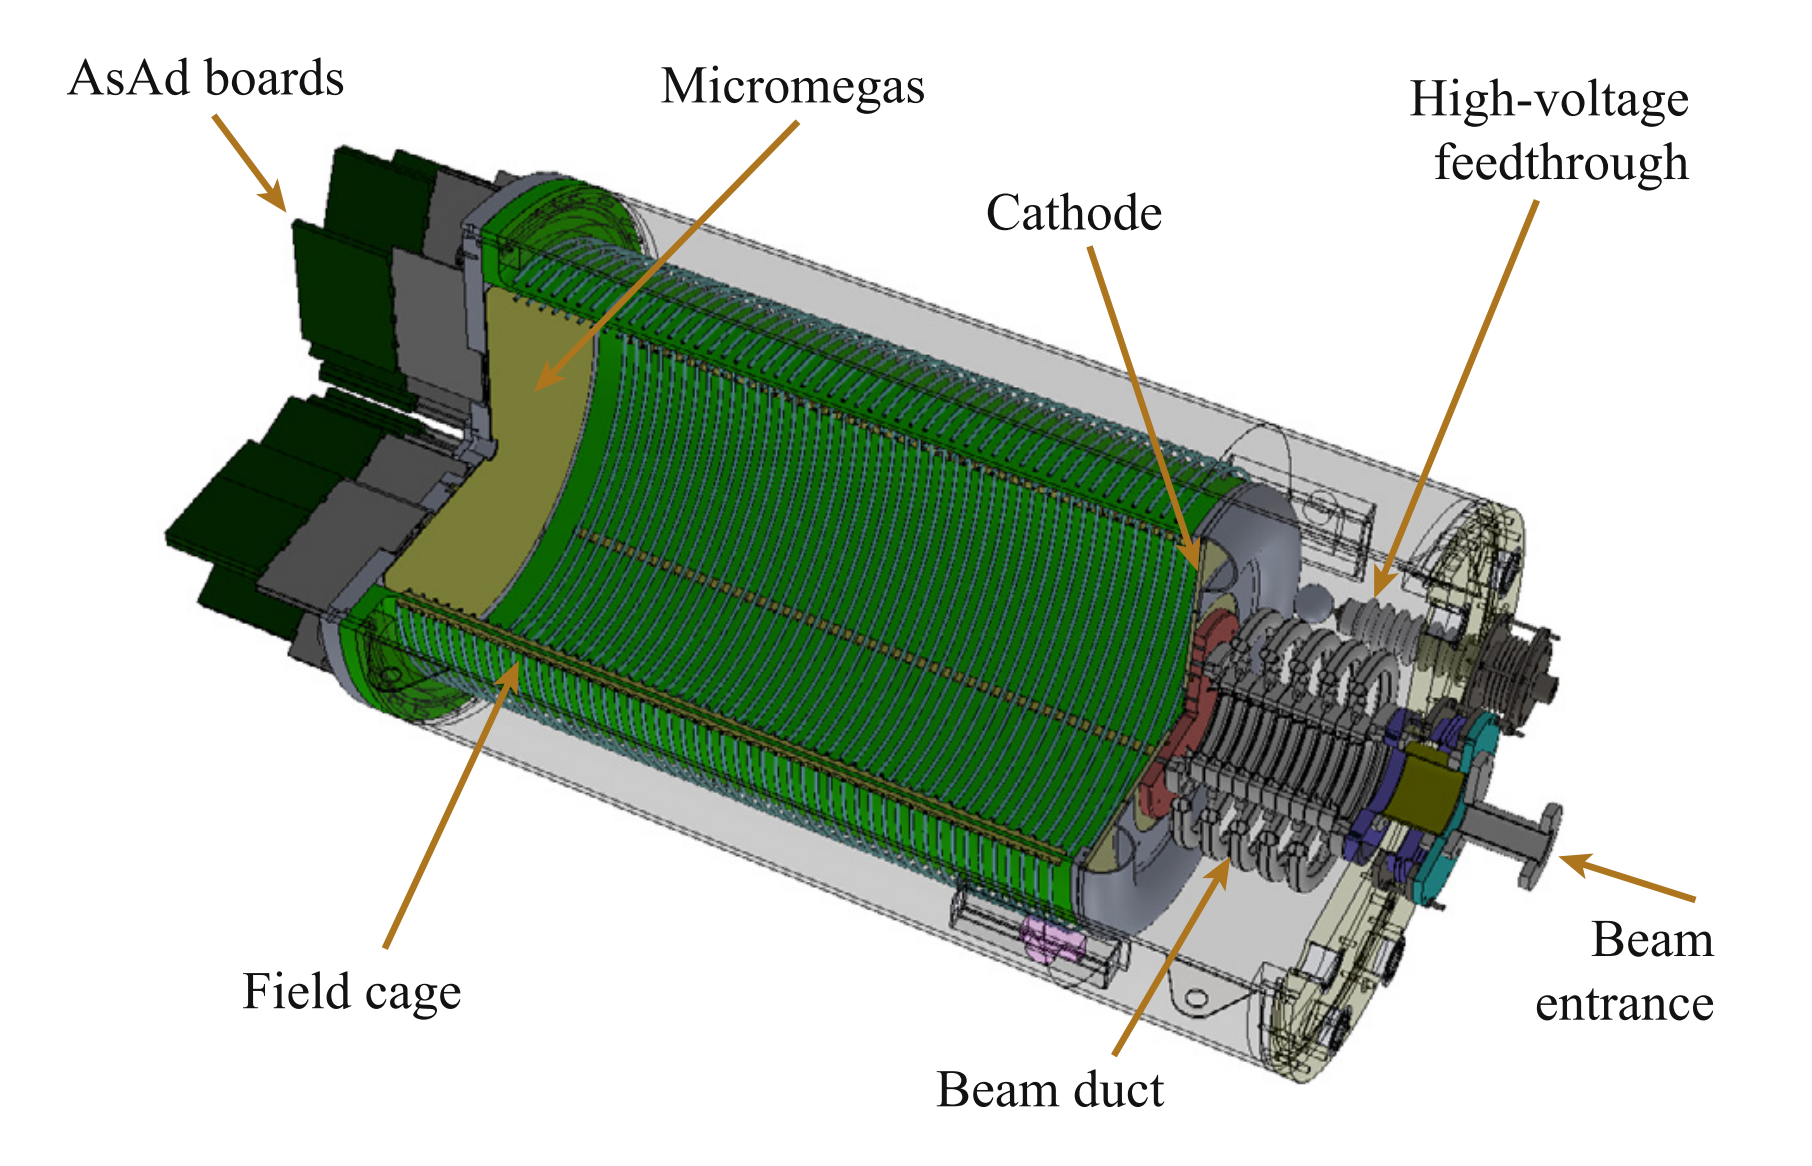
\includegraphics[height=3cm]{../chapters/experimental_background/plots/at_tpc_schematic.png}
		\caption{Diagram of the AT-TPC \footcite{Bradt2017a}}\label{fig:attpc}
	\end{figure}
	The AT-TPC is an experiment set up at the rare isotopes facility on the Michigan State University campus. The AT-TPC is commissioned to capture reactions with exotic nuclei.
\end{frame}

\begin{frame}[t]{AT-TPC}
	\begin{figure}
		\centering
		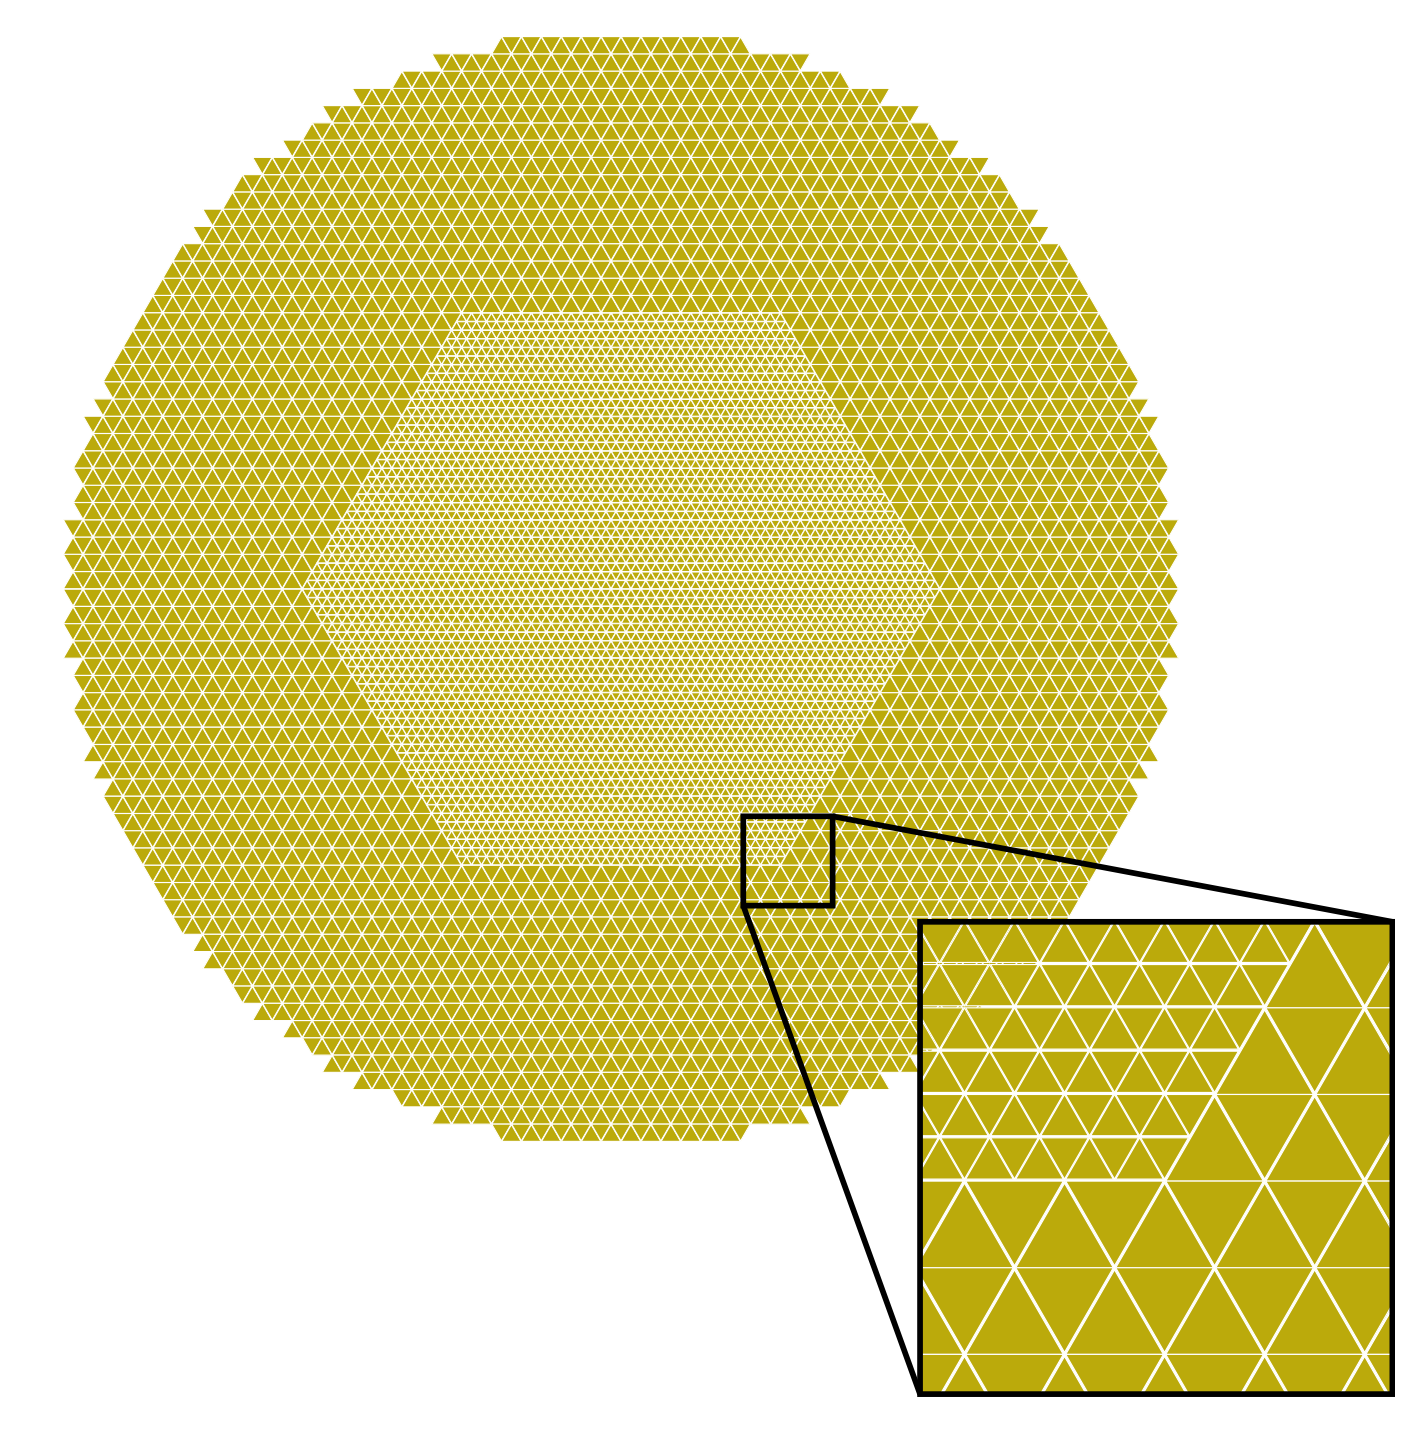
\includegraphics[height=3cm]{../chapters/experimental_background/plots/at_tpc_padplane.png}
		\caption{Detector pad plane of the AT-TPC \footcite{Bradt2017a}}\label{fig:padplane}
	\end{figure}
	Each triangle represents spatial discrete regions of the detector surface. The pad-plane consists of some $10^4$ sensor pads on a circle with $r=29cm$
\end{frame}

\begin{frame}[t]{AT-TPC Data}
	\begin{figure}[t]
		\centering
		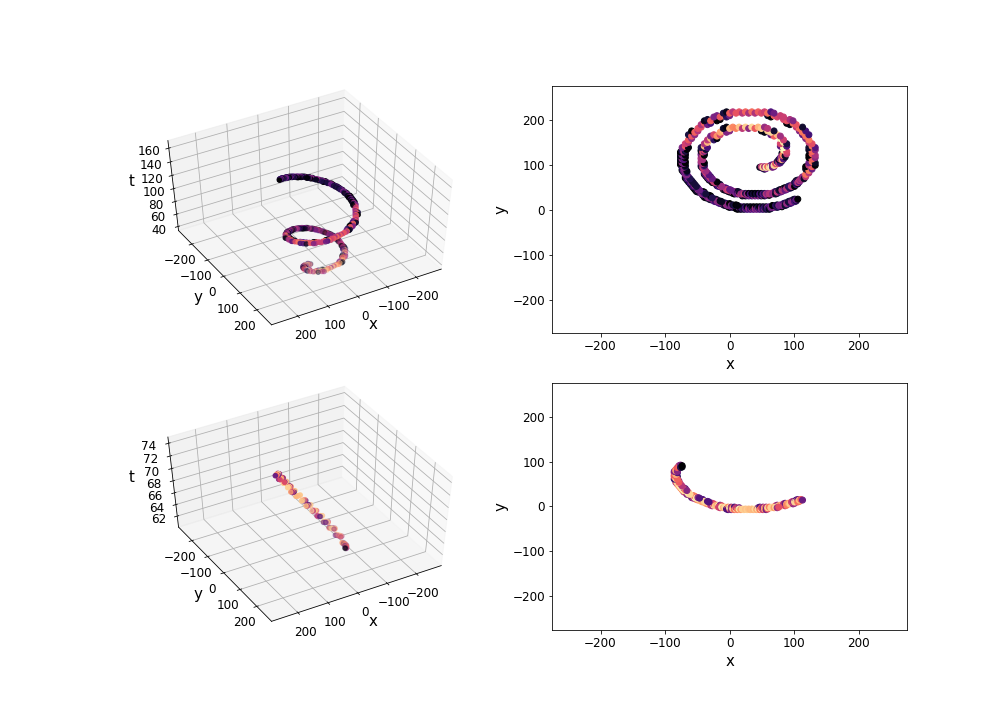
\includegraphics[width=0.8\linewidth]{../chapters/experimental_background/plots/display_eventssimulated.png}
		\caption{Simulated AT-TPC data in an experiment with ${}^{46}$Ar}
		\label{fig:name}
	\end{figure}
\end{frame}

\begin{frame}[t]{AT-TPC Data}
	\begin{figure}
		\subfloat[Unfiltered events from the ${}^{46}$Ar experiment]{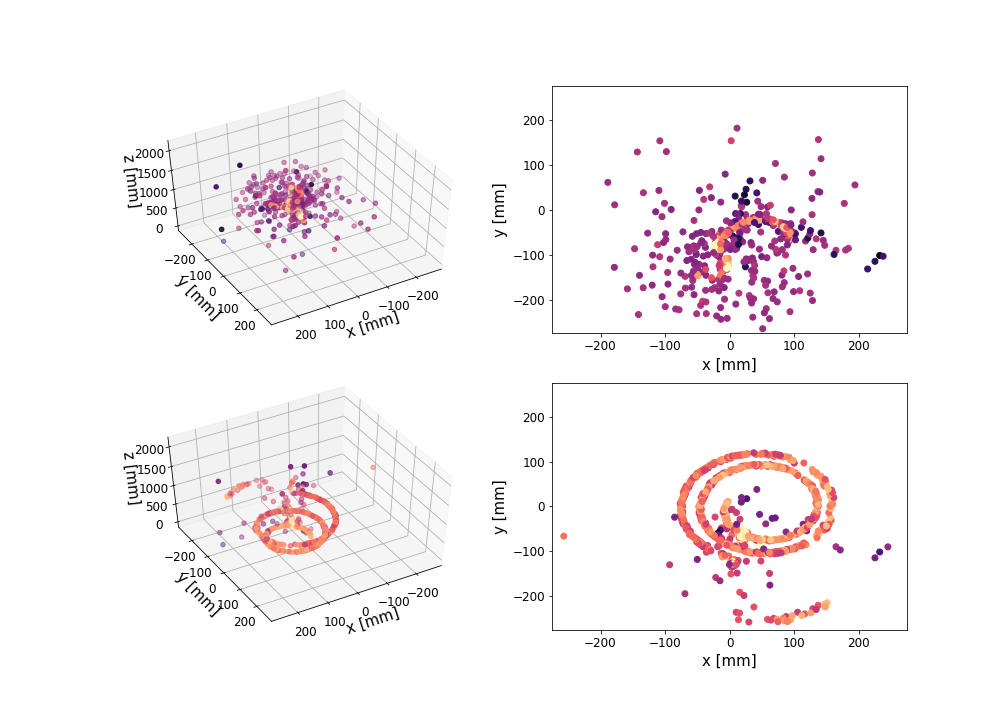
\includegraphics[width=0.4\linewidth]{../chapters/experimental_background/plots/display_eventsfull_.png}}
		\subfloat[Noise-filtered events from the ${}^{46}$Ar experiment]{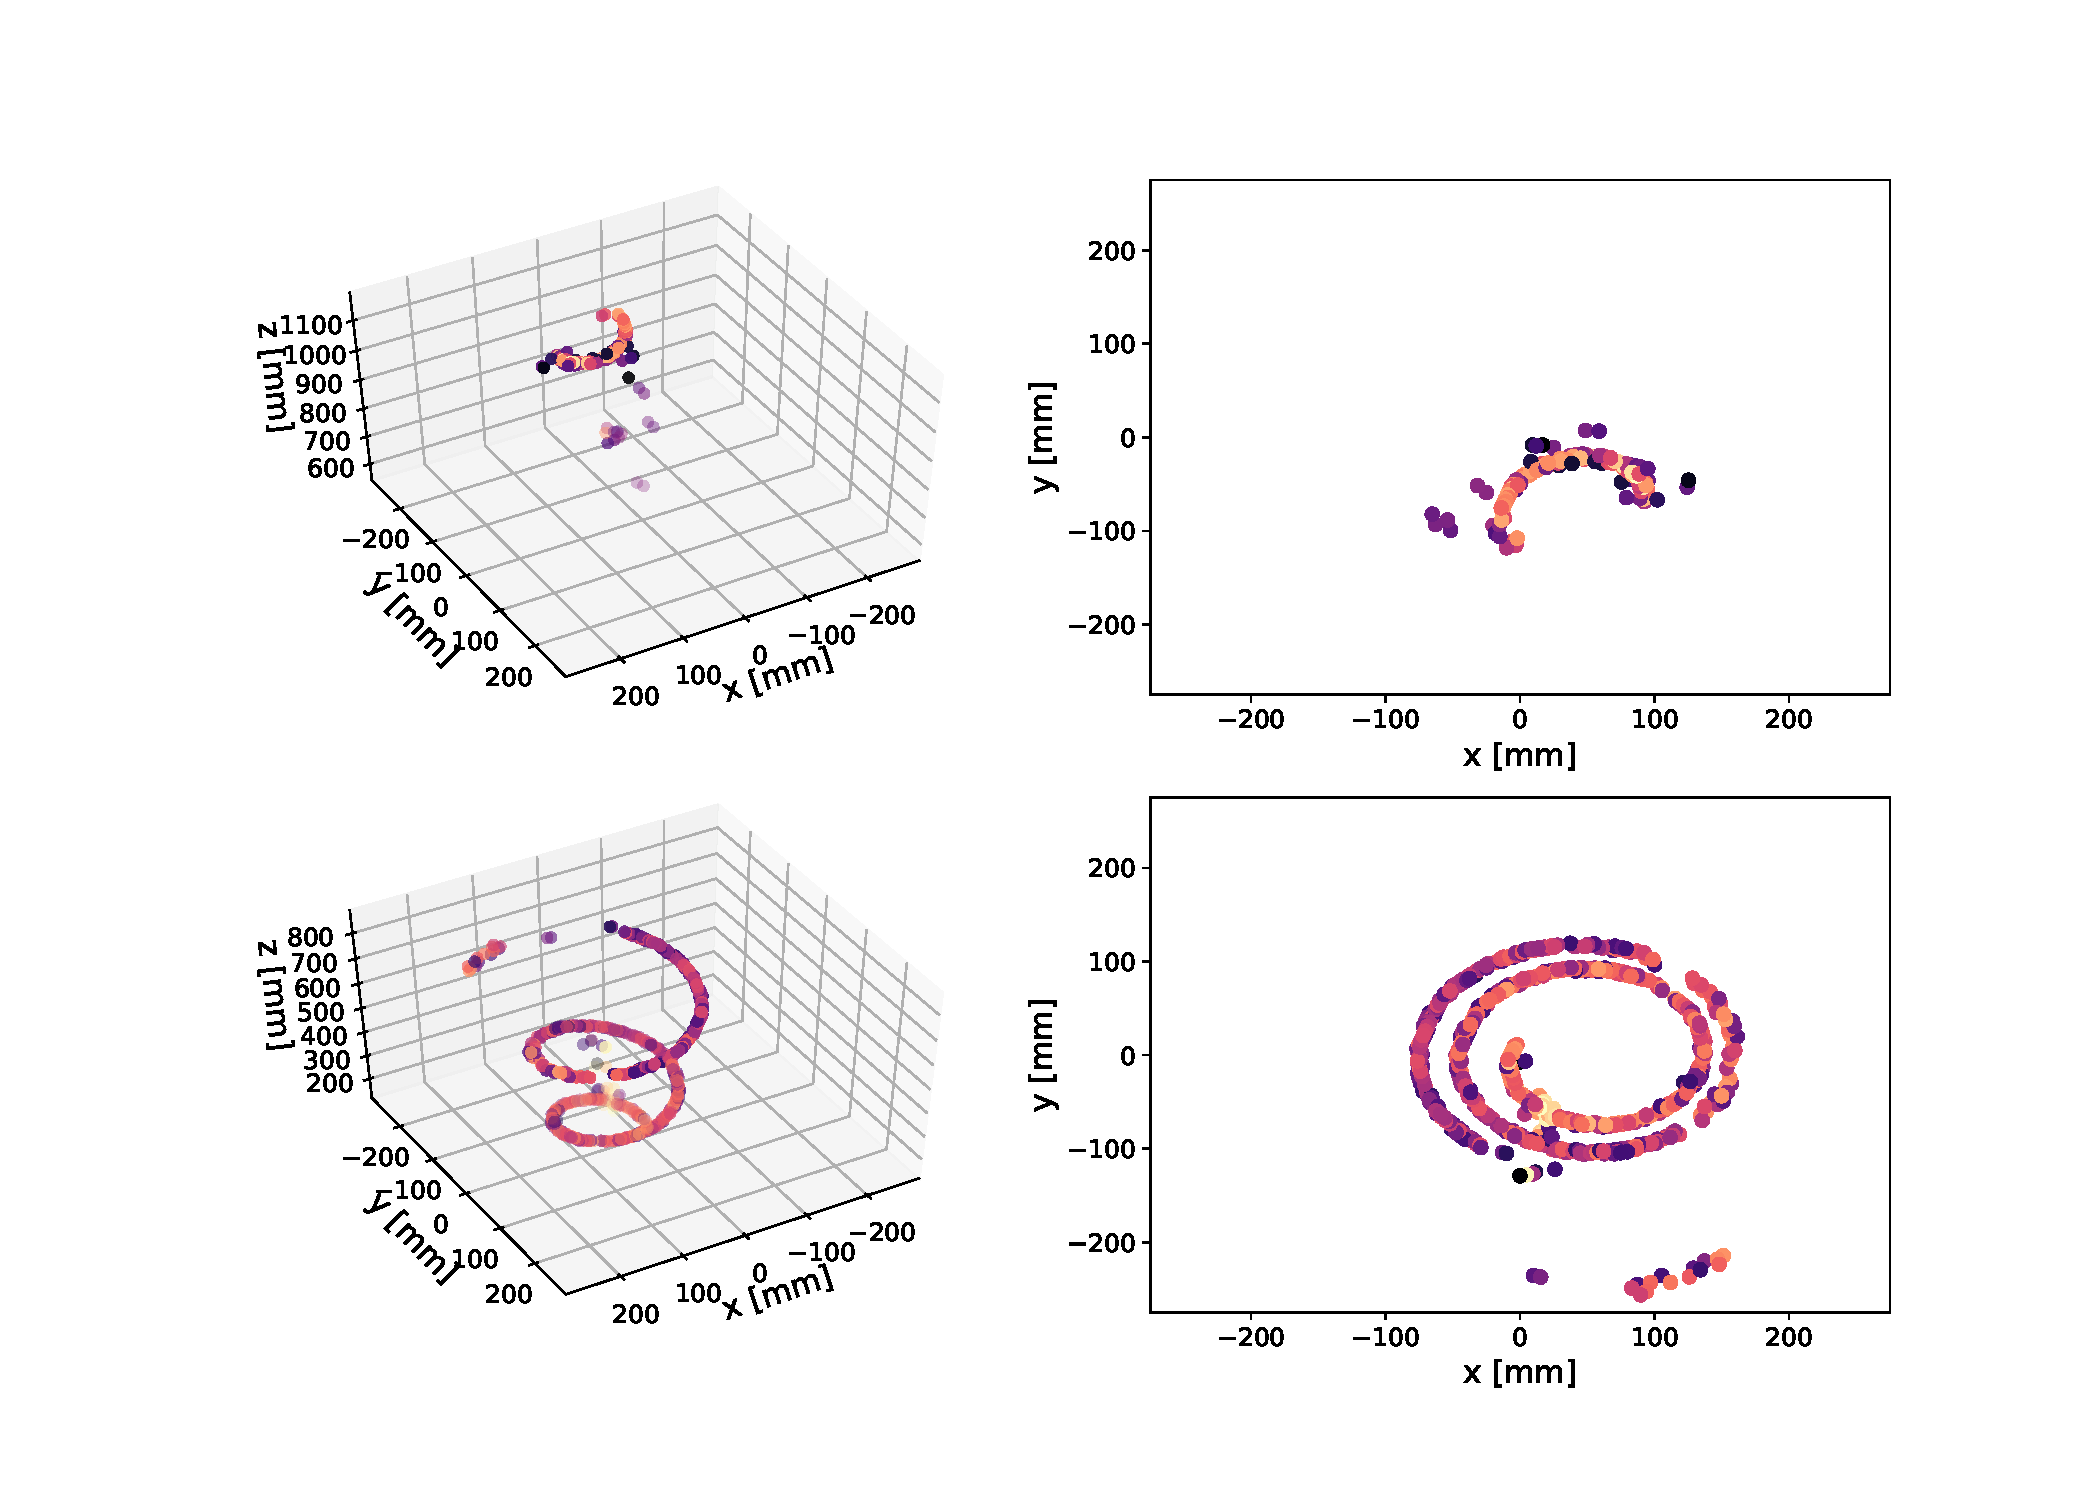
\includegraphics[width=0.5\linewidth]{../chapters/experimental_background/plots/display_eventsclean_.pdf}}
	\end{figure}
	Significant noise levels in the experiment, from unknown sources. Some $60\%$ of the recorded events are from unidentified reactions.
\end{frame}

\begin{frame}[t]{Challenges with the AT-TPC}
	\begin{enumerate}[I]
		\item Expensive integration - for each event a fit is computed
		\item Assumptions of the integration technique: 
			\begin{enumerate}[(i)]
				\item Each event is fit against parameters of the event of interest
				\item The integration is sensitive to Noise and Breaks in the tracks
			\end{enumerate}
	\end{enumerate}
	The amount of data is also significant: the experiment generates on the order of $10^5$ events per hour running.
	\begin{block}{Idea}
		Solve the problem by training deep neural networks, a very flexible algorithm from the Machine Learning community.
	\end{block}
\end{frame}

\begin{frame}[t]{Previous Work}
	\begin{itemize}
		\item Work on applying ML to this data started with a supervised learning project by Kuchera et al.\footcite{Kuchera2019}.
		\item The authors explored a \textit{supervised classification} problem of identifying reactions when ground-truth labels available.
		\item By fine tuning pre-trained networks the authors achieve very impressive performance.
	\end{itemize}
	One of the open questions is then, can we segment the events based on reactions without the ground truth labels?
\end{frame}

\begin{frame}[t]{ML background}
	Machine Learning (ML) is an amorphous set of algorithms for pattern recognition and function approximation. Bred as a mix between computer science and statistical learning theory, it includes algorithms like: 
	\begin{enumerate}[I]
		\item Linear Regression
		\item Logistic Regression
		\item Random Forest Classifiers
		\item Genetic Algorithms 
	\end{enumerate}
	And many others...
\end{frame}

\begin{frame}[t]{Deep Learning}
	A special sub-branch of Machine Learning is the field of Deep Learning, or more broadly: Differentiable Programming

	The premise of Deep Learning is to formulate an approximation to some unknown function $f(\mathbf{x})$ with a model, $\hat{f}$, that maintains some set of parameters $\{\theta\}$. 

	Some examples of the unknown function, $f(\mathbf{x})$, we would want to approximate are:
	\begin{enumerate}[(a)]
		\item a Hamiltonian of a system 
		\item a function which determines the thermodynamic phase of a system
		\item a function which itentifies dog-species from a picture
	\end{enumerate}
\end{frame}

\begin{frame}[t]{Deep Learning}
	Then then model can be tuned with gradient methods, the simplest of which is a steepest descent update: 
	\begin{equation}
		\theta_i \leftarrow \theta_i - \eta \frac{\partial \mathcal{C}(\mathbf{x}, f, \hat{f})}{\partial \theta_i},
	\end{equation}
	moderated by a \textit{learning rate} $\eta$ to ensure that the steps are small enough.

	The functional $\mathcal{C}$ is the \textit{cost} function for the problem and is commonly a variation of either, the Mean Squared Error: 

	\begin{equation}
		\mathcal{C}(\mathbf{x}, f, \hat{f}) = \sum (f(\mathbf{x})_i - \hat{f}(\mathbf{x})_i)^2,
	\end{equation}

	or the Cross Entropy

	\begin{equation}
		\mathcal{C}(\mathbf{x}, f, \hat{f}) = -\sum f(\mathbf{x})_i \log \hat{f}(\mathbf{x})_i. 
	\end{equation}
\end{frame}

\begin{frame}[t]{Deep Learning: Neural Networks}
	\begin{figure}[h]
		\centering
		\includegraphics[width=0.4\linewidth]{../chapters/theory/figures/ann.pdf}
		\caption{A neural network with three input nodes, two hidden nodes, and one output node}
		\label{fig:ann}
	\end{figure}
	Each of the \textit{activations} $\mathbf{a}$ are computed as a matrix product fed through a nonlinear activation \textit{activation function} g
	\begin{equation}\label{eq:fwd}
		\boldsymbol{a}^{[1]} = g(\boldsymbol{x}\boldsymbol{\theta}^{[1]})_D
	\end{equation}
\end{frame}

\begin{frame}[t]{Autoencoders}
	\begin{itemize}
		\item Recall that we want to separate classes of reaction products
		\item Additionally - we assume that we have access to very little or no ground truth labelled data
	\end{itemize}
	\begin{block}{ Idea }
		Learn the distribution over the events through two nonlinear maps which compress and inflate a representation of the events.
	\end{block}
	\begin{block}{Central Hypothesis}
		If we can compress a representation of an event reconstruct it - the compression must be informative of the type of event.
	\end{block}
\end{frame}

\begin{frame}[t]{Autoencoders}
	\begin{figure}[h]
		\centering
		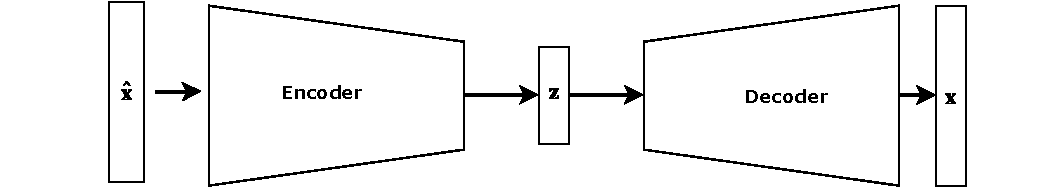
\includegraphics[width=0.8\linewidth]{../chapters/theory/autoencoder/plots/autoencoder.pdf}
		\caption{Autoencoder neural network schematic}%
		\label{fig:autoenc}
	\end{figure}

	An autoencoder is defined by an encoder/decoder pair of neural networks. We construct these such that 
	\begin{align}
		\text{dim}(\mathbf{\hat{x}}) \gg \text{dim}(\mathbf{z}),
	\end{align}

	and with the optimization objective
	\begin{align}
		\mathcal{O} = \text{arg min} || \mathbf{\hat{x}} - \text{Decoder}(\text{Encoder}(\mathbf{\hat{x}}))||_2 ^2.
	\end{align}
\end{frame}

\begin{frame}[t]{Experiment}
	\begin{itemize}
		\item We chose to represent the data as 2D projections, neglecting the z-axis.
		\item An autoencoder network is then fit to the events in an end to end manner.
		\item After traing, we extract the compressed (or \textit{latent}) expressions of the data.
		\item With varying amounts of labelled ground-truth data we fit a very simple classifier to the latent expressions
	\end{itemize}
	We wish to construct latent spaces that are as close to trivially separable, and so use a logistic regression classifier.
\end{frame}

\begin{frame}[t]{Results}
	\begin{figure}[h]
		\subfloat[Performance for an autoencoder with a naive architecture]{\includegraphics[height=3.5cm]{../chapters/results/classification/plots/ac_n_samples.pdf}}
		\subfloat[Performance using a representation of the events as seen by a VGG16 network]{\includegraphics[height=3.5cm]{../chapters/results/classification/plots/vgg_ac_n_samples.pdf}}
	\end{figure}
\begin{equation}\label{eq:recall}
\text{recall}= \frac{TP}{TP + FP}, \quad
\text{precision} = \frac{TP}{TP + FN}.
\end{equation}

\noindent The $f1$ score is defined as the harmonic mean of precision and recall for each class. Formally we define it as

\begin{equation}\label{eq:f1}
f1 = 2 \frac{\text{precision} \cdot \text{recall}}{\text{precision} + \text{recall}}.
\end{equation}
\end{frame}

\end{document}
